\section{Hardware demonstration}

The method runs on today's processors without realizing the number-non-conserving operator $\hat
c^\dagger_p$ on the device. One prepares a \emph{number-conserving} $(N{+}1)$-electron reference---a
Slater or local-unitary-cluster-Jastrow state with $n_\alpha=N/2+1$---and Trotter-evolves it
shallowly, mapping on-site interactions to native fractional $R_{ZZ}$ gates and hopping to Givens
rotations (Fig.~\ref{fig:circ}). Computational-basis bitstrings are sampled, recovered to the correct
particle-number sector by self-consistent configuration recovery~\cite{robledomoreno2025}, and the
entire $\hat c^\dagger_p$/Lehmann construction of Eq.~\eqref{eq:green} is assembled classically to
yield the full matrix $A_{pq}(\omega)$. Only a few Trotter steps are needed, because the classical
diagonalization is variational in the sampled subspace.

\begin{figure}[htbp]\centering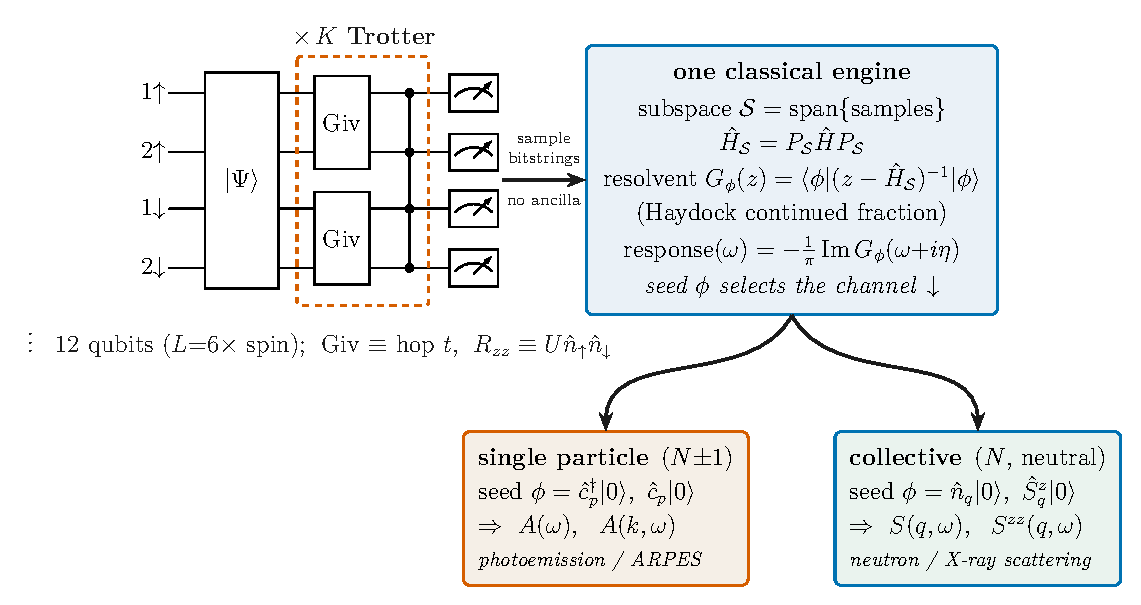
\includegraphics[width=\textwidth]{figs/fig_circuit.pdf}
\caption{\textbf{One sampling primitive, four dynamical responses.} A shallow, ancilla-free
circuit---state preparation and a Trotter layer repeated $K$ times (Givens rotations for the hopping
$t$, native $R_{zz}$ for the on-site $U\hat n_\uparrow\hat n_\downarrow$)---is measured in the
computational basis; no Hadamard test or controlled unitary is run on the device. The sampled
bitstrings define a sector-specific subspace $\mathcal S$ and feed a single classical engine---a Haydock
continued-fraction resolvent~\cite{haydock1972} $G_\phi(z)=\langle\phi|(z-\hat H_{\mathcal S})^{-1}|\phi\rangle$, whose
single-particle case ($\phi=\hat c^\dagger_p|0\rangle$) is the Green's function of
Eq.~\eqref{eq:green}. The seed $\phi$ then selects the channel: particle addition/removal seeds
$\hat c^{\dagger}_p|0\rangle,\hat c_p|0\rangle$ in the $(N{\pm}1)$ sectors give the single-particle
spectral functions $A(\omega)$ and $A(k,\omega)$ (photoemission/ARPES), while number-conserving density
and spin seeds $\hat n_q|0\rangle,\hat S^z_q|0\rangle$ in the $N$ sector give the dynamical structure
factors $S(q,\omega)$ and $S^{zz}(q,\omega)$ (neutron/X-ray scattering)---all from \emph{one} sampling
primitive, the seed selecting the sector and hence the subspace. The four channels are realized in Figs.~\ref{fig:method} ($A(\omega)$),
\ref{fig:lattice} ($A(k,\omega)$), \ref{fig:sqw} ($S(q,\omega)$), and \ref{fig:spin}
($S^{zz}(q,\omega)$).}\label{fig:circ}\end{figure}

Executed on the IBM Heron processor \texttt{ibm\_fez} for the $L=6$ Hubbard model at $U/t=4$ (broadening
$\eta=0.15\,t$; $12$ qubits; the $t=0$ reference plus $K=7$ real-time-evolution circuits, whose $50{,}000$
pooled computational-basis shots define the union subspace; TREX readout twirling, Pauli twirling, and
dynamical decoupling, and \emph{no} zero-noise extrapolation), the bitstring-sampled spectral function
reproduces the exact $A(\omega)$ to within the line-broadening resolution
(Fig.~\ref{fig:heron})---a demonstration on a real quantum computer that the open-gap method works.
At this scale the $(N{+}1)$ sector is small enough that hardware sampling with self-consistent
recovery captures essentially the complete subspace; the robustness underlying this clean result is
quantified under a per-qubit bit-flip channel: self-consistent configuration recovery holds the
spectral reconstruction near relative-$L_1\approx0.05$ out to $\varepsilon\approx16\%$, far beyond the
naive-post-selection range where the error grows steadily with the flip rate (Fig.~\ref{fig:noise}). The demonstration realizes time-evolved QSCI~\cite{teqsci2024} and
sample-based Krylov diagonalization~\cite{skqd2025,kirby2023,yoshioka2025} lifted into the
$(N{\pm}1)$ sectors; the nearest published sibling also builds a subspace from
sampled configurations---from short-time quantum-evolved states with classically projected long-time
dynamics---but targets the \emph{neutral}-sector molecular response, not the charged-$(N{\pm}1)$
single-particle Green's function our Lehmann construction assembles~\cite{santini2025}; the hardware Green's-function and dynamical-structure-factor
results of the trapped-ion line~\cite{greenediniz2024,quantinuum_dsf2026} use non-subspace routes.
A ready-to-run notebook for the $\mathrm{N_2}$ molecular spectral function---a
double-factorized Trotter of the molecular Hamiltonian feeding the same sample--recover--Lehmann
pipeline, \emph{not executed on hardware here}---is provided as an ancillary file, bridging the concept from the Hubbard model to
chemistry and situating the method within the quantum-centric-supercomputing program that couples IBM
Heron processors to the Fugaku supercomputer~\cite{robledomoreno2025,shirakawa2025} under
error-mitigated observable estimation~\cite{qesem2025,algorithmiq2026}.

To take the same sample--recover pipeline to a molecular energy, we ran the ground state of stretched
$\mathrm{N_2}$ ($R=2.0$~\AA, valence active space) on a second Heron processor,
\texttt{ibm\_marrakesh} ($10{,}000$ shots), through a double-factorized Trotter circuit. Self-consistent
configuration recovery reaches, averaged over $8$ recovery seeds on the same device counts,
$E_{\mathrm{hw}}=-108.80745\pm0.00014$~Ha---$0.59\pm0.14$~mHa of the exact FCI value
($E_{\mathrm{FCI}}=-108.80804$~Ha; best seed $0.40$~mHa)---well below chemical accuracy on a real device
for a strongly multireference bond (Fig.~\ref{fig:heron}, panel~b). Notably, the same shallow circuit evaluated by \emph{noiseless} statevector
simulation lands at $-108.77850$~Ha ($29.5$~mHa error): here the device noise, filtered through recovery,
populates valid configurations the ideal shallow circuit misses, an instance of the noise-assisted
recovery mechanism we analyze at length in a companion study~\cite{review}. The same effect has been
reported independently on a variable-length cuprate chain, where real trapped-ion noise \emph{improves}
the sample-based energy convergence over the noiseless statevector simulation~\cite{wray2025}, and---on
$\mathrm{N_2}$ with the LUCJ ansatz, the present system---the same noise-enhanced configuration recovery
is reported independently in~\cite{vaquero2026}, so the mechanism is not an artifact of one processor or
one molecule. The quoted $\pm0.14$~mHa is the spread over the $8$ recovery
seeds---the stochastic uncertainty of the self-consistent recovery on the fixed device counts, not a
device-repeat statistic; the systematic version, across nineteen molecules and a controlled noise model, is the subject of
Fig.~\ref{fig:noiserec} below.

\paragraph{Why $\mathrm{N_2}$ alone is not the test: noise robustness across chemistry.} A single
molecule cannot separate a genuine mechanism from a lucky geometry, so we stress-test the
sample--recover energy pipeline across the entire nineteen-molecule suite of
Table~\ref{tab:molecules} under a controlled, hardware-motivated noise model. For each dissociated
molecule we Born-sample the exact ground-state configuration distribution, apply an independent
per-qubit bit-flip channel at rate $\varepsilon$, and rebuild the subspace either by naive
in-sector post-selection or by self-consistent configuration recovery (S-CoRe) to the correct $(N_\alpha,N_\beta)$
sector; the recovered configurations are diagonalized and the energy is compared to FCI, seed-averaged
(Fig.~\ref{fig:noiserec}). Two facts emerge, and both bound the limits. First, at a
realistic Heron-scale rate $\varepsilon=2\%$ the subspace energy is intrinsically forgiving---because
diagonalization in the sampled subspace is variational, corrupted bitstrings that survive as valid
configurations only enlarge the subspace, a valid-shot economy rather than a fidelity gain---so $18/19$ molecules reach chemical accuracy with recovery
(the lone exception is the strongly multireference $\mathrm{H_6}$ chain at $3.6$~mHa), and S-CoRe
converts one of the two naive failures ($\mathrm{NH_3}$, $2.65\!\to\!1.51$~mHa) into a success. Second, and
more informative, the \emph{advantage} of recovery grows monotonically with the noise: where naive
post-selection discards the increasing fraction of out-of-sector strings and its error climbs steeply
($\mathrm{N_2}$: $0.4\!\to\!6.4\!\to\!31.9$~mHa at $\varepsilon=0,20,30\%$), S-CoRe reassigns them to
physical configurations and roughly halves the error throughout ($\mathrm{N_2}$: $0.4\!\to\!3.3\!\to
\!13.2$~mHa; $\mathrm{CO}$ actually \emph{improves}, from $1.7$~mHa at $\varepsilon=0$ to a $0.6$~mHa
minimum near $\varepsilon=20\%$ ($0.7$~mHa at $\varepsilon=30\%$), as recovered strings enrich
the subspace). The effect is molecule-dependent: species whose ground state concentrates on few
determinants ($\mathrm{C_2}$) are essentially noise-immune out to $\varepsilon=30\%$ ($\mathrm{H_2O}$ is
likewise noise-immune at the realistic $\varepsilon=2\%$),
while the hardest ($\mathrm{H_6}$) remains the residual challenge---consistent with the resource
analysis of Sec.~\ref{sec:resource}, where the cost is the determinant support $|\mathcal S|$---tracked by the entanglement, not predicted by one-body magic.
This is the molecular counterpart of the Hubbard noise sweep of Fig.~\ref{fig:noise}, and it answers
the natural objection to a single-molecule hardware run: the recovery mechanism is a property of the
chemistry, not of $\mathrm{N_2}$.

\begin{figure}[htbp]\centering% fragment: \input into the figure environment -> \normalsize equals the body font exactly.
\definecolor{inkPrim}{HTML}{1B1B1B}\definecolor{inkMute}{HTML}{6E6E6E}
\definecolor{warmFill}{HTML}{E8770C}\definecolor{warmLine}{HTML}{7A1E10}
\definecolor{hwWarm}{HTML}{C4360C}\definecolor{simSlate}{HTML}{9AA1AC}\definecolor{band}{HTML}{ECE7DF}
\begin{tikzpicture}[font=\rmfamily]
\pgfplotsset{hpanel/.style={width=8.5cm,height=6.0cm,axis line style={inkPrim,line width=0.6pt},
  tick style={inkPrim,line width=0.6pt},tick label style={font=\normalsize},label style={font=\normalsize},
  title style={font=\normalsize,yshift=1pt},ymajorgrids,major grid style={inkMute,opacity=0.10,line width=0.3pt}}}
% ===================== (a) ibm_fez : spectral function A(omega) =====================
% CLEAN: curve + title only; all technical detail (shots, mitigation, coverage) lives once, in the caption.
\begin{axis}[name=axa,hpanel,
  title={(a)\ \ \texttt{ibm\_fez} $\cdot$ 12 qubits: \ $A(\omega)$},
  xlabel={frequency \ $\omega-E_0$}, ylabel={$A(\omega)$},
  xmin=2.31,xmax=21.02,ymin=0,ymax=0.603]
  \addplot[draw=none,fill=warmFill,fill opacity=0.28] table[x=w,y=A]{figs/heron_hot.dat} \closedcycle;
  \addplot[warmLine,line width=1.3pt] table[x=w,y=A]{figs/heron_hot.dat};
\end{axis}
% ===================== (b) ibm_marrakesh : N2 ground-state energy =====================
% CLEAN: two curves + which-is-which + the two headline numbers; specs/jobs live once, in the caption.
\begin{axis}[name=axb,hpanel,at={(axa.south east)},anchor=south west,xshift=1.4cm,
  title={(b)\ \ \texttt{ibm\_marrakesh} $\cdot$ 24 qubits: \ $\mathrm{N_2}$ energy},
  xlabel={configuration-recovery step}, ylabel={error to FCI \ (mHa)},
  ymode=log,xmin=-0.35,xmax=4.55,ymin=0.28,ymax=90,
  xtick={0,1,2,3,4},ytick={0.5,1,3,10,30},yticklabels={$0.5$,$1$,$3$,$10$,$30$}]
  \fill[band,opacity=0.72] (axis cs:-0.35,0.28) rectangle (axis cs:4.55,1.6);
  \node[anchor=south west,font=\normalsize,inkPrim] at (axis cs:-0.28,0.42) {chem.\ accuracy};
  \addplot[simSlate,line width=1.4pt,dash pattern=on 5pt off 3pt,mark=square,mark size=2.6pt,
           mark options={draw=simSlate,fill=white,line width=1pt}] coordinates {(0,31.17) (1,29.60) (2,29.55) (3,29.55)};
  % REAL hardware recovery trajectory (hist_hw from hw_lucj_n2_result.json: [-108.781038,...] -> [27.00,6.99,2.49,1.10] mHa);
  % the converged final point is the 8-seed mean 0.59+-0.14 mHa (the only per-seed statistic available) -> capped error bar there only.
  \addplot[hwWarm,line width=2.2pt,mark=*,mark size=3.0pt,mark options={fill=hwWarm,draw=white,line width=0.7pt}]
     coordinates {(0,27.00) (1,6.99) (2,2.49) (3,1.10) (4,0.588)};
  \addplot[hwWarm,only marks,mark=*,mark size=3.2pt,mark options={fill=hwWarm,draw=white,line width=0.8pt},
     error bars/.cd,y dir=both,y explicit,error bar style={hwWarm,line width=1.1pt},
     error mark=-,error mark options={rotate=90,hwWarm,line width=1.1pt,mark size=4pt}]
     coordinates {(4,0.588)+-(0,0.142)};
  % which curve is which: a leader from each label lands ON its own curve; plus the two headline numbers
  \node[anchor=south,font=\normalsize,inkPrim] (nl) at (axis cs:1.85,44)
    {noiseless (same circuit), $29.5$~mHa};
  \draw[-{Stealth[length=1.7mm]},inkPrim,line width=0.5pt] (nl.south) -- (axis cs:1.55,30.0);
  \node[anchor=south,align=center,font=\normalsize,inkPrim] (nh) at (axis cs:3.05,5.2)
    {noisy hardware\\$0.59\pm0.14$~mHa};
  \draw[-{Stealth[length=1.7mm]},inkPrim,line width=0.5pt] (nh.south) -- (axis cs:3.0,1.15);
\end{axis}
\end{tikzpicture}

\caption{\textbf{The complete quantum-hardware record of this work: two runs on IBM~Heron processors.}
\textbf{(a)}~Single-particle spectral function $A(\omega)$ of the $L=6$ Hubbard model at $U/t=4$,
$\eta=0.15\,t$ ($12$ qubits; the classical validation of Fig.~\ref{fig:method} is a different instance,
$U/t=8$), reconstructed from $50{,}000$ computational-basis bitstrings sampled on \texttt{ibm\_fez} (TREX
readout twirling, Pauli twirling, and dynamical decoupling). The device histogram
covered the complete $(N{+}1)$ sector ($|\mathcal S|\!=\!300/300$), so the reconstruction is exact by
coverage---a proof of principle, not a fidelity or beyond-classical claim.
\textbf{(b)}~Ground-state energy error of stretched $\mathrm{N_2}$ ($R=2.0$~\AA, CAS(10e,12o)/cc-pVDZ,
$24$ qubits) versus self-consistent configuration-recovery step, on \texttt{ibm\_marrakesh} ($10{,}000$ shots,
double-factorized Trotter circuit). The noisy device (solid) reaches
$0.59\pm0.14$~mHa of the exact FCI value---well below chemical accuracy---whereas the noiseless statevector
simulation of the \emph{same} shallow circuit (dashed) is stranded at $29.5$~mHa: device noise, filtered
through configuration recovery, populates valid configurations the ideal shallow circuit misses. The
solid curve is the mean over $8$ recovery seeds on the cached device counts; the shaded envelope and the
capped whiskers at every step both show the $\pm1$~s.d.\ spread across those $8$ seeds (widest at
step~$0$, $31.1\pm4.0$~mHa, where it starts together with the noiseless curve, and tapering as recovery
converges to $0.59\pm0.14$~mHa; best seed $0.40$~mHa). The
systematic version across nineteen molecules under a controlled noise model is Fig.~\ref{fig:noiserec}. These two runs are the entirety of the quantum
hardware used here; every other result in this work is an exact classical simulation.}\label{fig:heron}\end{figure}

\begin{figure}[htbp]\centering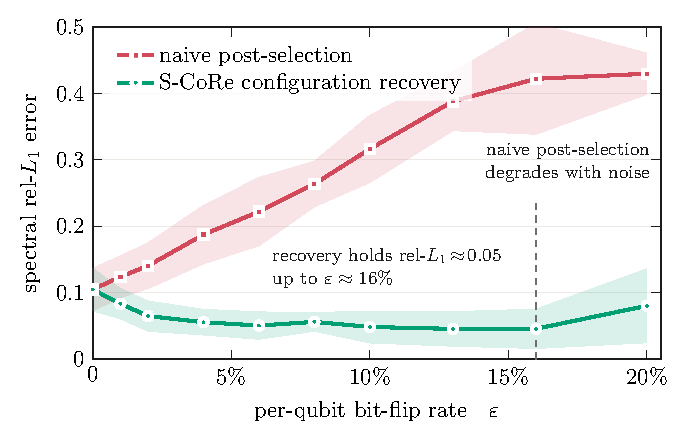
\includegraphics[width=0.7\textwidth]{figs/fig_noise_score.pdf}
\caption{\textbf{Noise robustness (synthetic per-qubit bit-flip channel, $L=6$).} Spectral
relative-$L_1$ error vs the per-qubit bit-flip rate $\varepsilon$, applied to bitstrings Born-sampled from
the exact distribution (this is a controlled classical simulation, not a device run). Naive
post-selection degrades steadily, whereas S-CoRe self-consistent configuration recovery holds the error
near $0.05$ out to $\varepsilon\approx16\%$ (seed-averaged over $6$ seeds at $6{,}000$ shots each; bands
$=\pm1$ s.d.\ across seeds).}\label{fig:noise}\end{figure}

\begin{figure}[htbp]\centering% self-contained native pgfplots fragment (fig:noiserec)
\definecolor{nrH6}{HTML}{6A4C93}
\definecolor{nrNH3}{HTML}{E8880C}
\definecolor{nrN2}{HTML}{D7263D}
\definecolor{nrCO}{HTML}{12876F}
\definecolor{nrC2}{HTML}{2E6F95}
\definecolor{nrOK}{HTML}{0E7C7B}\definecolor{nrBad}{HTML}{5E4B8B}\definecolor{nrNv}{HTML}{D1495B}\definecolor{nrChem}{HTML}{2E7D32}
\begin{tikzpicture}
\begin{groupplot}[group style={group size=2 by 1, group name=nrg, horizontal sep=1.45cm}, height=9.5cm, paperaxis,
  title style={at={(0,1)},anchor=south west,font=\bfseries,yshift=1pt}]
\nextgroupplot[width=0.505\linewidth, ymode=log, xmin=-1, xmax=31, ymin=3e-3, ymax=80,
  xlabel={per-qubit bit-flip rate $\varepsilon$ (\%)}, ylabel={energy error vs FCI (mHa)}, title={(a)},
  legend style={at={(0.5,0.03)},anchor=south,font=\normalsize,draw=black!20},legend columns=3,legend cell align=left]
\draw[nrChem,dashed,line width=0.6pt] (axis cs:-1,1.6) -- (axis cs:31,1.6);
% chemical-accuracy label: emitted after the groupplot, see below.
\addplot[name path=H6lo,draw=none,forget plot] coordinates {(0,3.2914) (2,3.0066) (5,3.6550) (10,3.7659) (15,5.3712) (20,8.9720) (30,15.6267)};
\addplot[name path=H6hi,draw=none,forget plot] coordinates {(0,4.5041) (2,4.1385) (5,4.4412) (10,6.5199) (15,9.5780) (20,16.7961) (30,29.8587)};
\addplot[nrH6,opacity=0.15,forget plot] fill between[of=H6lo and H6hi];
\addplot[name path=NH3lo,draw=none,forget plot] coordinates {(0,2.1436) (2,1.4495) (5,1.0457) (10,0.7919) (15,1.3563) (20,1.8046) (30,5.7326)};
\addplot[name path=NH3hi,draw=none,forget plot] coordinates {(0,2.9078) (2,1.9853) (5,1.6281) (10,1.6847) (15,2.0580) (20,2.8561) (30,20.1868)};
\addplot[nrNH3,opacity=0.15,forget plot] fill between[of=NH3lo and NH3hi];
\addplot[name path=N2lo,draw=none,forget plot] coordinates {(0,0.1729) (2,0.1550) (5,0.3169) (10,0.2965) (15,0.6158) (20,1.4642) (30,8.4636)};
\addplot[name path=N2hi,draw=none,forget plot] coordinates {(0,0.6006) (2,0.6093) (5,0.6846) (10,1.3158) (15,2.3324) (20,5.5026) (30,17.8734)};
\addplot[nrN2,opacity=0.15,forget plot] fill between[of=N2lo and N2hi];
\addplot[name path=COlo,draw=none,forget plot] coordinates {(0,1.5510) (2,1.5669) (5,1.0491) (10,0.7344) (15,0.5781) (20,0.4698) (30,0.3702)};
\addplot[name path=COhi,draw=none,forget plot] coordinates {(0,1.9155) (2,2.0418) (5,1.4264) (10,1.3026) (15,1.0358) (20,0.7942) (30,1.0249)};
\addplot[nrCO,opacity=0.15,forget plot] fill between[of=COlo and COhi];
\addplot[name path=C2lo,draw=none,forget plot] coordinates {(0,0.1703) (2,0.1351) (5,0.0827) (10,0.0677) (15,0.0479) (20,0.0385) (30,0.0118)};
\addplot[name path=C2hi,draw=none,forget plot] coordinates {(0,0.1967) (2,0.1807) (5,0.1240) (10,0.0817) (15,0.0730) (20,0.0627) (30,0.0433)};
\addplot[nrC2,opacity=0.15,forget plot] fill between[of=C2lo and C2hi];
\addplot[nrH6,line width=1.4pt,mark=*,mark size=1.3pt,mark options={fill=nrH6,draw=white,line width=0.4pt}] coordinates {(0,3.8978) (2,3.5726) (5,4.0481) (10,5.1429) (15,7.4746) (20,12.8840) (30,22.7427)}; \addlegendentry{H$_6$}
\addplot[nrH6,line width=0.9pt,densely dashed,forget plot] coordinates {(0,3.8978) (2,4.6251) (5,5.6347) (10,7.8697) (15,12.9901) (20,23.8560) (30,50.3837)};
\addplot[nrNH3,line width=1.4pt,mark=*,mark size=1.3pt,mark options={fill=nrNH3,draw=white,line width=0.4pt}] coordinates {(0,2.5257) (2,1.7174) (5,1.3369) (10,1.2383) (15,1.7072) (20,2.3304) (30,12.7391)}; \addlegendentry{NH$_3$}
\addplot[nrNH3,line width=0.9pt,densely dashed,forget plot] coordinates {(0,2.5257) (2,2.9622) (5,2.7617) (10,2.9227) (15,3.7294) (20,5.5505) (30,31.5152)};
\addplot[nrN2,line width=1.4pt,mark=*,mark size=1.3pt,mark options={fill=nrN2,draw=white,line width=0.4pt}] coordinates {(0,0.3843) (2,0.3445) (5,0.5007) (10,0.6589) (15,1.3685) (20,3.2538) (30,13.1685)}; \addlegendentry{N$_2$}
\addplot[nrN2,line width=0.9pt,densely dashed,forget plot] coordinates {(0,0.3843) (2,0.4335) (5,0.6929) (10,1.1118) (15,2.8006) (20,6.3706) (30,31.8749)};
\addplot[nrCO,line width=1.4pt,mark=*,mark size=1.3pt,mark options={fill=nrCO,draw=white,line width=0.4pt}] coordinates {(0,1.7332) (2,1.8043) (5,1.2377) (10,1.0185) (15,0.8069) (20,0.6320) (30,0.6975)}; \addlegendentry{CO}
\addplot[nrCO,line width=0.9pt,densely dashed,forget plot] coordinates {(0,1.7332) (2,1.9851) (5,1.9371) (10,1.4901) (15,1.8518) (20,2.5550) (30,2.8339)};
\addplot[nrC2,line width=1.4pt,mark=*,mark size=1.3pt,mark options={fill=nrC2,draw=white,line width=0.4pt}] coordinates {(0,0.1835) (2,0.1579) (5,0.1034) (10,0.0747) (15,0.0604) (20,0.0506) (30,0.0261)}; \addlegendentry{C$_2$}
\addplot[nrC2,line width=0.9pt,densely dashed,forget plot] coordinates {(0,0.1835) (2,0.1635) (5,0.1143) (10,0.0811) (15,0.0746) (20,0.0647) (30,0.0657)};
\nextgroupplot[width=0.425\linewidth, xmode=log, xmin=2.2e-3, xmax=14, enlarge y limits=0.03,
  ytick={0,1,2,3,4,5,6,7,8,9,10,11,12,13,14,15,16,17,18}, yticklabels={BeH$_2$,H$_2$,LiH,HF,F$_2$,H$_2$O,H$_4$,OH,LiF,BH,N$_2$,BeH,C$_2$,NO,O$_2$,CN,CO,NH$_3$,H$_6$}, y tick label style={font=\normalsize},
  xtick={0.01,0.1,1,10}, xticklabels={$0.01$,$0.1$,$1$,$10$}, xminorticks=false,
  xlabel={energy error at $\varepsilon=2\%$ (mHa)}, title={(b)},
  legend style={at={(0.03,0.03)},anchor=south west,font=\normalsize,draw=black!20},legend cell align=left]
\fill[nrChem,fill opacity=0.06] (axis cs:2.2e-3,-0.6) rectangle (axis cs:1.6,18.6);
\draw[nrChem,dashed,line width=0.7pt] (axis cs:1.6,-0.6) -- (axis cs:1.6,18.6);
\node[nrChem,font=\tiny,anchor=south,rotate=90] at (axis cs:1.6,9.5) {};
\draw[black!32,line width=0.8pt] (axis cs:0.0022,0) -- (axis cs:0.0022,0); \draw[black!32,line width=0.8pt] (axis cs:0.0022,1) -- (axis cs:0.0022,1); \draw[black!32,line width=0.8pt] (axis cs:0.0022,2) -- (axis cs:0.0022,2); \draw[black!32,line width=0.8pt] (axis cs:0.0022,3) -- (axis cs:0.0022,3); \draw[black!32,line width=0.8pt] (axis cs:0.0022,4) -- (axis cs:0.0022,4); \draw[black!32,line width=0.8pt] (axis cs:0.0327,5) -- (axis cs:0.0022,5); \draw[black!32,line width=0.8pt] (axis cs:0.3178,6) -- (axis cs:0.0022,6); \draw[black!32,line width=0.8pt] (axis cs:0.0194,7) -- (axis cs:0.0194,7); \draw[black!32,line width=0.8pt] (axis cs:0.0254,8) -- (axis cs:0.0254,8); \draw[black!32,line width=0.8pt] (axis cs:0.0845,9) -- (axis cs:0.0605,9); \draw[black!32,line width=0.8pt] (axis cs:0.0688,10) -- (axis cs:0.0636,10); \draw[black!32,line width=0.8pt] (axis cs:0.1367,11) -- (axis cs:0.1367,11); \draw[black!32,line width=0.8pt] (axis cs:0.1711,12) -- (axis cs:0.1615,12); \draw[black!32,line width=0.8pt] (axis cs:0.3275,13) -- (axis cs:0.1942,13); \draw[black!32,line width=0.8pt] (axis cs:0.4696,14) -- (axis cs:0.3363,14); \draw[black!32,line width=0.8pt] (axis cs:0.7815,15) -- (axis cs:0.7261,15); \draw[black!32,line width=0.8pt] (axis cs:1.3923,16) -- (axis cs:1.2450,16); \draw[black!32,line width=0.8pt] (axis cs:2.6491,17) -- (axis cs:1.5063,17); \draw[black!32,line width=0.8pt] (axis cs:4.3814,18) -- (axis cs:3.5606,18);
\addplot[only marks,mark=o,mark size=1.9pt,nrNv,line width=0.8pt] coordinates {(0.0022,0) (0.0022,1) (0.0022,2) (0.0022,3) (0.0022,4) (0.0327,5) (0.3178,6) (0.0194,7) (0.0254,8) (0.0845,9) (0.0688,10) (0.1367,11) (0.1711,12) (0.3275,13) (0.4696,14) (0.7815,15) (1.3923,16) (2.6491,17) (4.3814,18)}; \addlegendentry{naive}
\addplot[only marks,mark=*,mark size=2.1pt,nrOK] coordinates {(0.0022,0) (0.0022,1) (0.0022,2) (0.0022,3) (0.0022,4) (0.0022,5) (0.0022,6) (0.0194,7) (0.0254,8) (0.0605,9) (0.0636,10) (0.1367,11) (0.1615,12) (0.1942,13) (0.3363,14) (0.7261,15) (1.2450,16) (1.5063,17) (3.5606,18)}; \addlegendentry{S-CoRe}
\node[black,font=\normalsize,anchor=north east] at (axis cs:1.4720000000000002,18.3) {$1.6$ mHa};
\end{groupplot}
\node[nrChem,font=\footnotesize,anchor=south east,inner sep=1pt]
      at (nrg c1r1.north east) {chemical accuracy ($1.6$\,mHa)};
\end{tikzpicture}

\caption{\textbf{Noise-assisted SQD ground-state energy across the molecular suite.}
\textbf{(a)}~Energy error vs the per-qubit bit-flip rate $\varepsilon$ for five representative molecules
($\mathrm{H_6}$, $\mathrm{NH_3}$, $\mathrm{N_2}$, CO, $\mathrm{C_2}$; seed-averaged over $8$ seeds at $4{,}000$ shots each, bands $=\pm1$ s.d.\ across seeds; log scale). Solid $=$ S-CoRe recovery, dashed $=$ naive
post-selection. The recovery advantage grows with noise, and for $\mathrm{CO}$ and $\mathrm{C_2}$ the
recovered subspace drives the error \emph{below} the noiseless value; $\mathrm{C_2}$ is
effectively noise-immune across the full $\varepsilon$ sweep. \textbf{(b)}~The full nineteen-molecule suite at a realistic
$\varepsilon=2\%$ (log scale, sorted): for each molecule the naive post-selection error (open circle) is
linked to the S-CoRe value (filled), so the leftward pull is the recovery gain; the shaded band is
chemical accuracy ($<1.6$~mHa). Eighteen of nineteen land inside it; $\mathrm{H_6}$, the most
multireference case, is the residual challenge. Panels (a) and (b) are independent seed ensembles
(panel (a): $8$ seeds; panel (b): $5$ seeds, $4000$ shots), so a given molecule's $\varepsilon=2\%$ value
can differ by up to a factor of a few between them (for $\mathrm{N_2}$, $0.34$ vs $0.06$~mHa; both far below chemical accuracy).}\label{fig:noiserec}\end{figure}

\paragraph{Data and code availability.} Both hardware runs are archived with full metadata. For each run
we provide, as ancillary files, the raw measurement counts, the transpiled circuits (OpenQASM), the
backend, calibration date, physical-qubit layout and coupling map, transpiled two-qubit-gate count and
depth, job identifiers, the reference-state (LUCJ/Slater) parameters, the Trotter step and the
real-time-evolution times $t_k=k\,\Delta t$ ($k=0,\dots,7$: the $t=0$ reference plus the $K=7$ evolutions)
that define the union subspace, and the full mitigation settings (TREX, Pauli twirling, dynamical decoupling). The scripts that regenerate every
figure and Table~\ref{tab:molecules}---including the per-molecule geometries, active spaces, FCI energies,
absolute $|\mathcal S|$, sector dimension $D$, and minimal bond dimension $\chi$ of
App.~\ref{app:repro}---are provided alongside; every non-hardware result is an exact classical simulation
reproducible from them.
